\section{Results and discussion}




\revise{}
{
\subsection{Computational results}\label{sec_computational_results}
}
We evaluate the proposed framework and the various beading schemes on a set of different types of 3D models, ranging over various applications and various types of geometry. 
The data set is described in Appendix~\ref{dataset}.
We sliced all models in the data set and selected 300 random slices for analysis.
Toolpaths of these 300 outline shapes are generated using the uniform technique as implemented by Clipper~\cite{johnson2014clipper} -- a state-of-the-art polygon offset library,
and by our framework using four beading schemes, i.e. the constant bead count scheme with a bead count of $C=4$, the centered, the evenly distributed, and the inward distributed beading scheme using $N=3$, all with a preferred bead width\revise{s}{} of $w^* = \SI{0.4}{\milli\meter}$.
The tests were performed on a desktop PC equipped with an Intel Core i7-7500U CPU @ \SI{2.70}{\giga\hertz} (a single core is used) and \SI{16.3}{\giga\byte} memory.







\subsubsection{Accuracy}
We first evaluate the accuracy of different beading schemes in terms of the relative amount of the overfill and underfill. 
\begin{wrapfigure}{r}{.3\columnwidth}
\centering
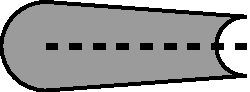
\includegraphics[width=.25\columnwidth]{sources-validation-visualization-principle-rounded-excluded-single.pdf}
\caption{
Extrusion segments coverage.
The hole at the end will be filled by the next extrusion segment.
}
\label{segment_visualization_simple}
\end{wrapfigure}
We construct the over- and underfill area by comparing the shapes covered by each extrusion move (\cref{segment_visualization_simple}) with each other and with the total shape of the boundary polygons. (For implementation details see Appendix~\ref{accuracy_calculation}.)
This results in polygonal shapes such as visualized in the top half of \cref{visualized_accuracy}:
there are orange shapes where the beads overlap and azure shapes in the voids in between the beads.


We compare the total area in \si{\milli\meter\squared} of these overfill and underfill shapes to the total area of the boundary for each sample in the data set
and report the average percentages in see \cref{over_underfill}.
The inward distributed scheme has a calculated overfill of \SI{0.24}{\percent} and an underfill of \SI{0.17}{\percent}.
This is lower compared to the uniform scheme, which results in \SI{1.2}{\percent} overfill and \SI{1.7}{\percent} underfill in the data set.

\begin{figure*}
\centering
\setlength{\figwidth}{0.19\textwidth}
\setlength{\figheight}{0.283\textwidth}
\begin{subfigure}{\figwidth}\centering
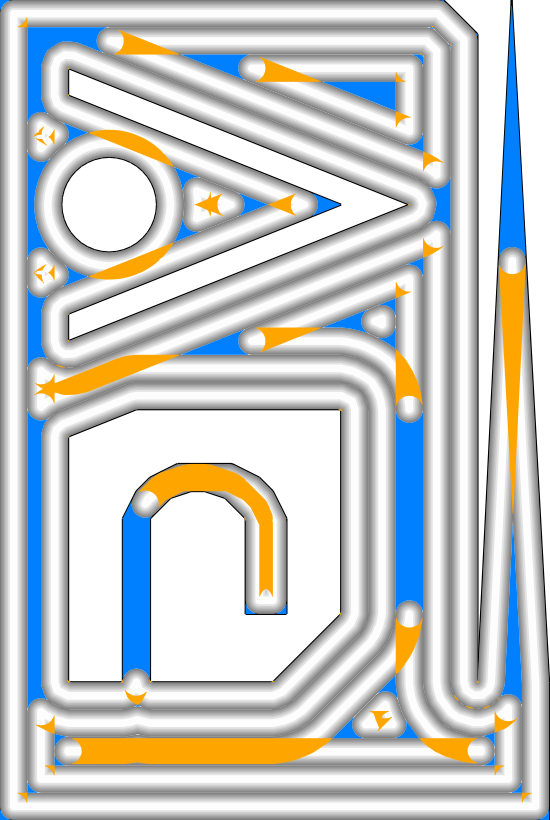
\includegraphics[height=\figheight]{sources-validation-gMAT-example-TEST-naive-accuracy.png}
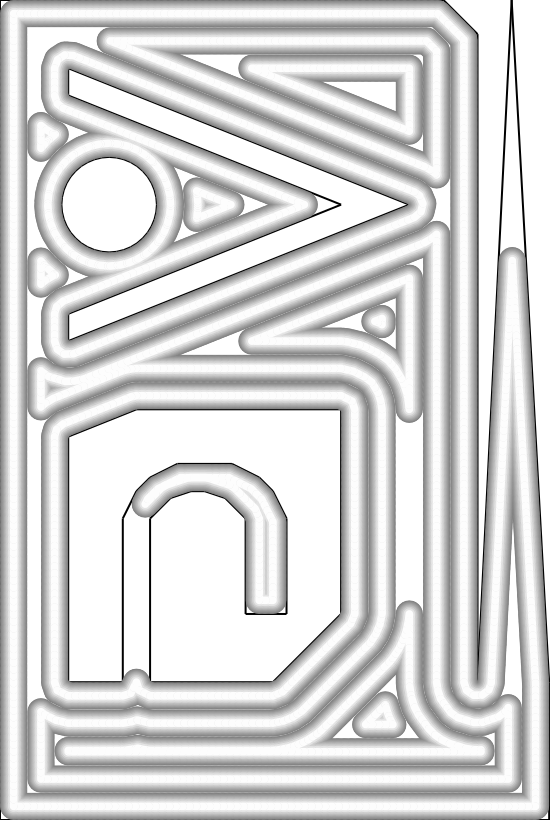
\includegraphics[height=\figheight]{sources-validation-gMAT-example-TEST-naive-widths.png}
\caption{Uniform}\label{TEST_naive_accuracy}
\end{subfigure}
%\begin{subfigure}{\figwidth}\centering
%\includegraphics[height=\figheight]{sources-validation-gMAT-example-TEST-SingleBead-accuracy.png}
%\includegraphics[height=\figheight]{sources-validation-gMAT-example-TEST-SingleBead-widths.png}
%\caption{Single}\label{TEST_SingleBead_accuracy}
%\end{subfigure}
\begin{subfigure}{\figwidth}\centering
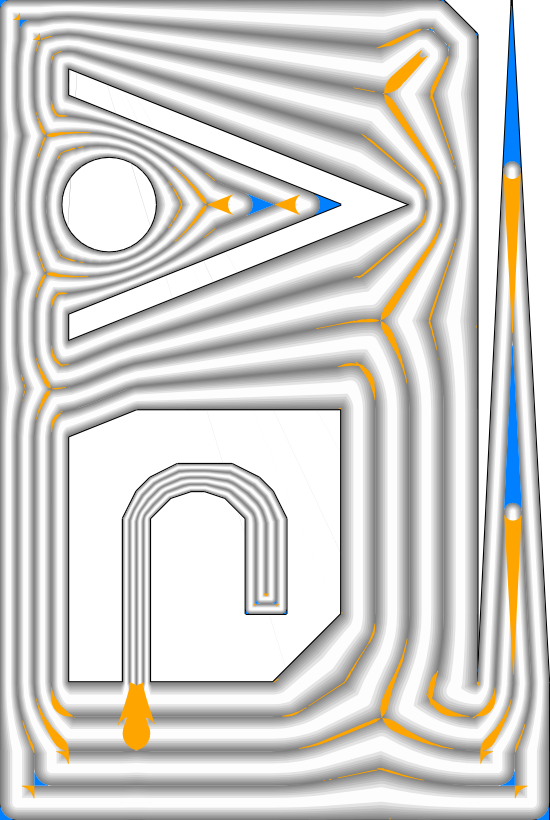
\includegraphics[height=\figheight]{sources-validation-gMAT-example-TEST-Constant-accuracy.png}
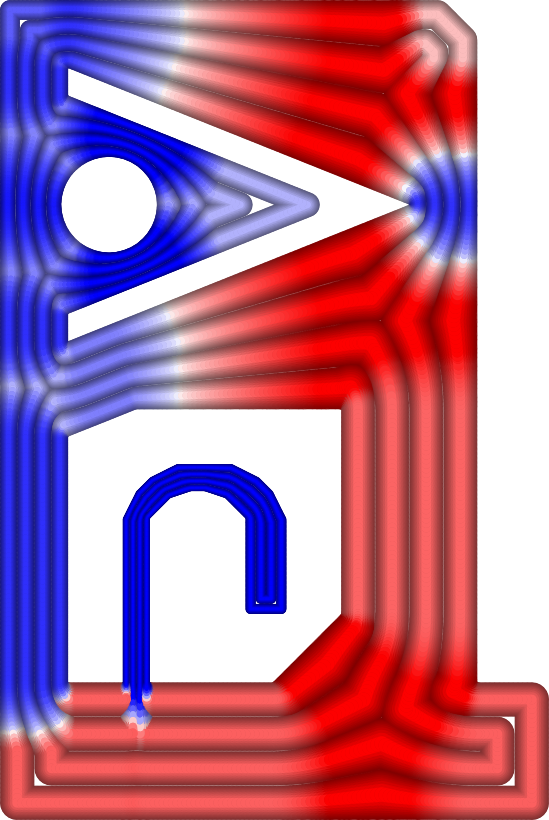
\includegraphics[height=\figheight]{sources-validation-gMAT-example-TEST-Constant-widths.png}
\caption{Constant}\label{TEST_Constant_accuracy}
\end{subfigure}
\begin{subfigure}{\figwidth}\centering
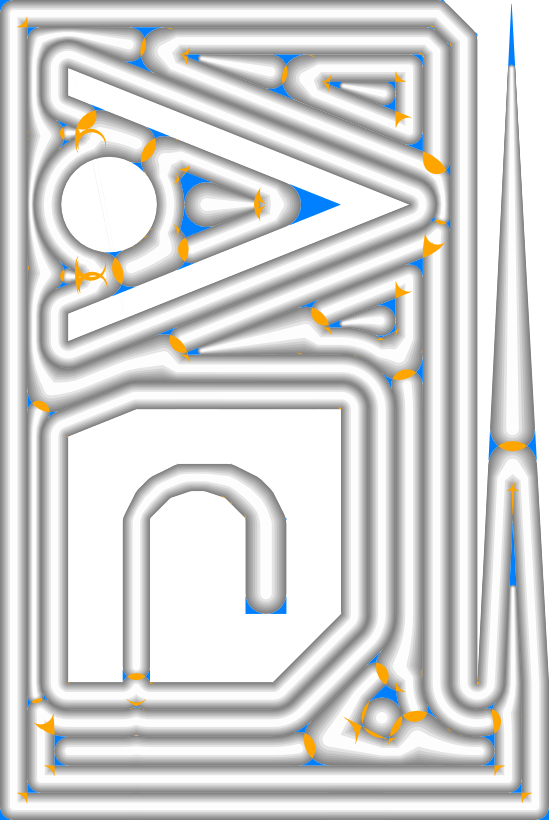
\includegraphics[height=\figheight]{sources-validation-gMAT-example-TEST-Center-accuracy.png}
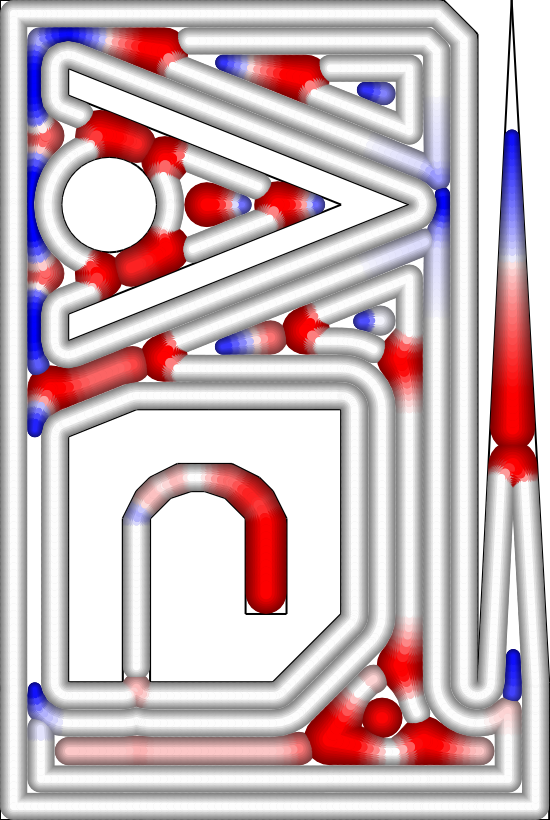
\includegraphics[height=\figheight]{sources-validation-gMAT-example-TEST-Center-widths.png}
\caption{Centered}\label{TEST_Center_accuracy}
\end{subfigure}
\begin{subfigure}{\figwidth}\centering
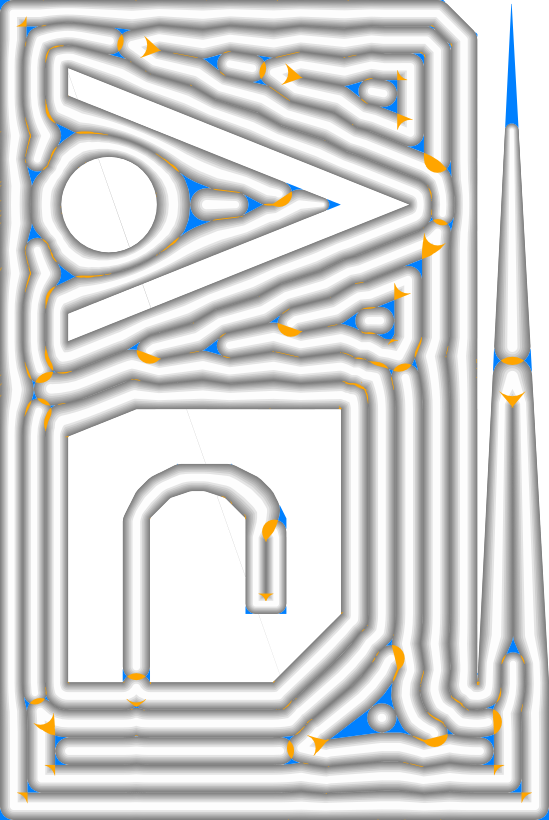
\includegraphics[height=\figheight]{sources-validation-gMAT-example-TEST-Distributed-accuracy.png}
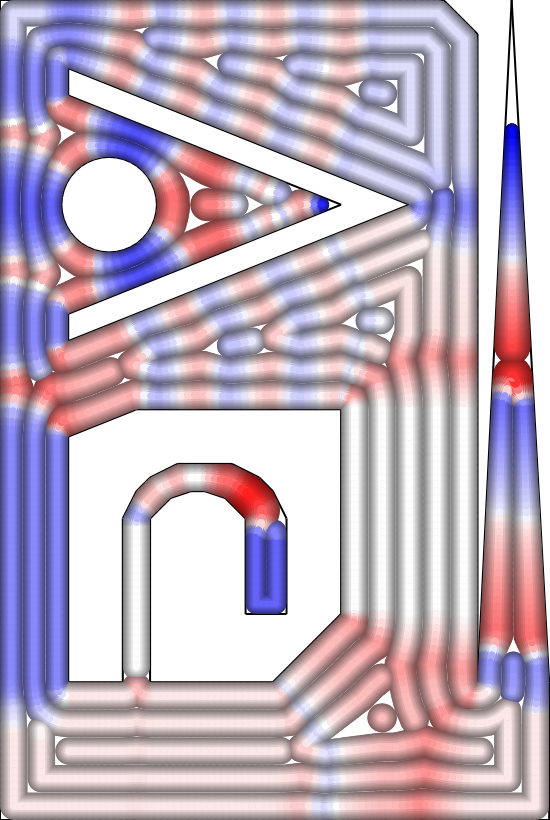
\includegraphics[height=\figheight]{sources-validation-gMAT-example-TEST-Distributed-widths.png}
\caption{Distributed}\label{TEST_Distributed_accuracy}
\end{subfigure}
\begin{subfigure}{\figwidth}\centering
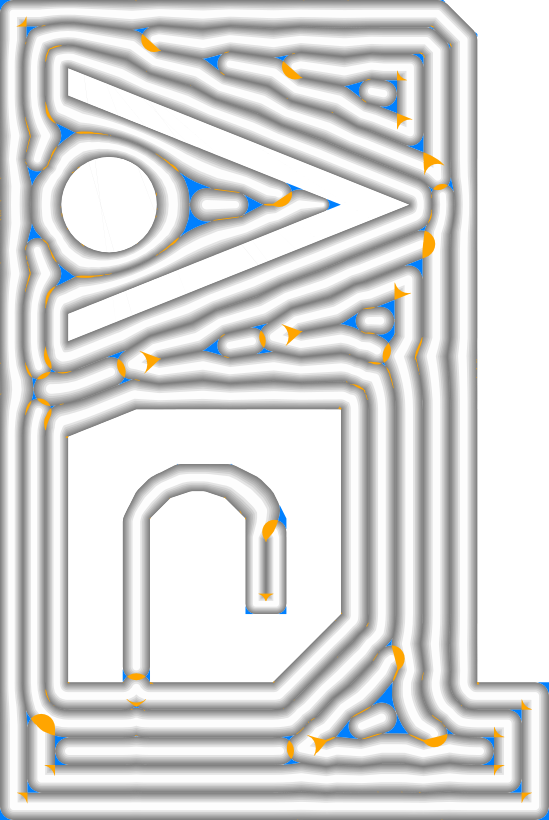
\includegraphics[width=\columnwidth]{sources-validation-gMAT-example-TEST-InwardDistributed-accuracy.png}
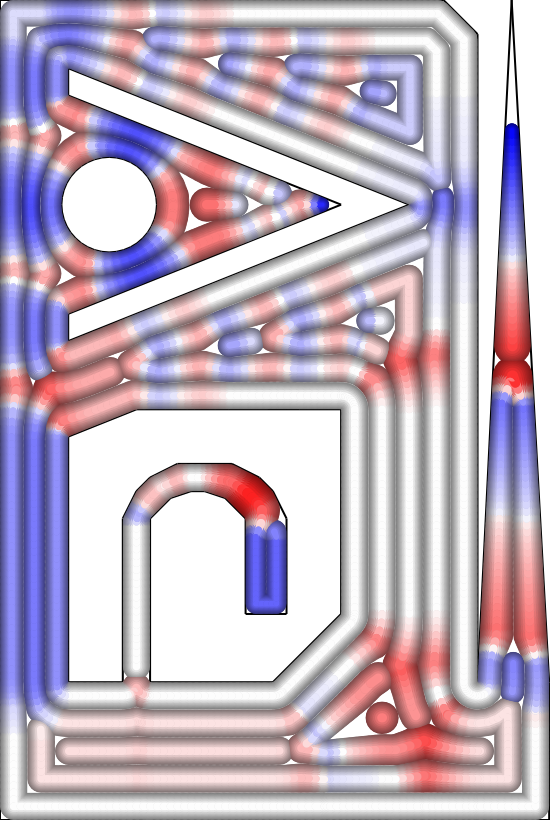
\includegraphics[width=\columnwidth]{sources-validation-gMAT-example-TEST-InwardDistributed-widths.png}
\caption{Inward \revise{}{($N=2$)}}\label{TEST_InwardDistributed_accuracy}
\end{subfigure}
\begin{subfigure}{.04\columnwidth}\centering
\vspace{4.7cm}
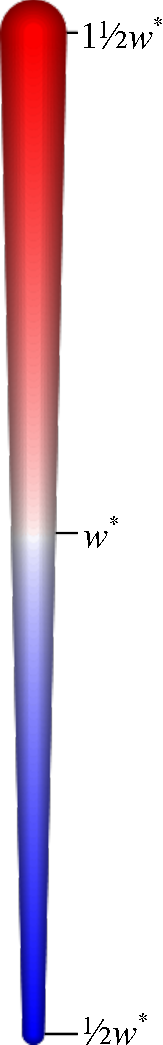
\includegraphics[height=\figheight]{sources-validation-gMAT-example-widths-legend.pdf}
\end{subfigure}
\caption{
Visualization of the overfills and underfills (top) and the widths (bottom) for various beading schemes.
Extrusion beads in gray tones,
overfill in orange,
underfill in azure,
narrow beads in blue
and wide beads in red.
\revise{New shape contains pointy wedge to see impact on minimal feature size}{In order to distinguish clearly from the Distributed scheme the Inward is limited to $N=2$.}
}
\label{visualized_accuracy}
\end{figure*}




\begin{figure*}
\centering
\setlength{\figheight}{0.22\textwidth}
\setlength{\figwidth}{0.31\textwidth}
\begin{subfigure}{\figwidth}\centering
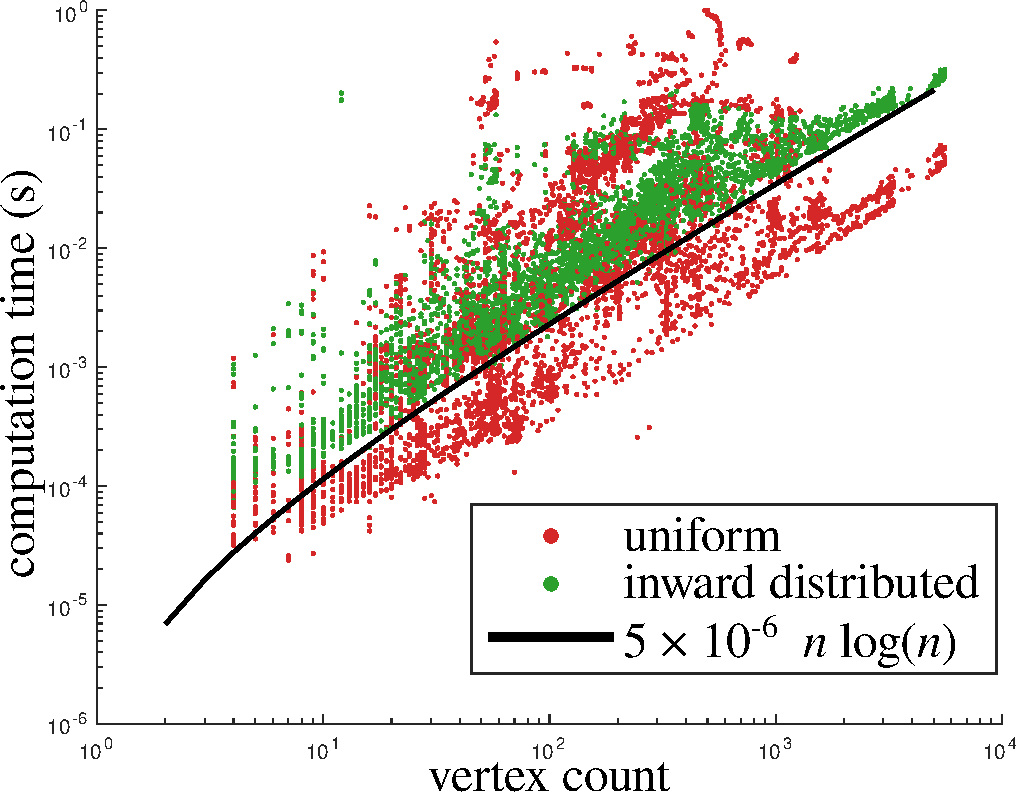
\includegraphics[height=\figheight]{sources-validation-computime2.pdf}
%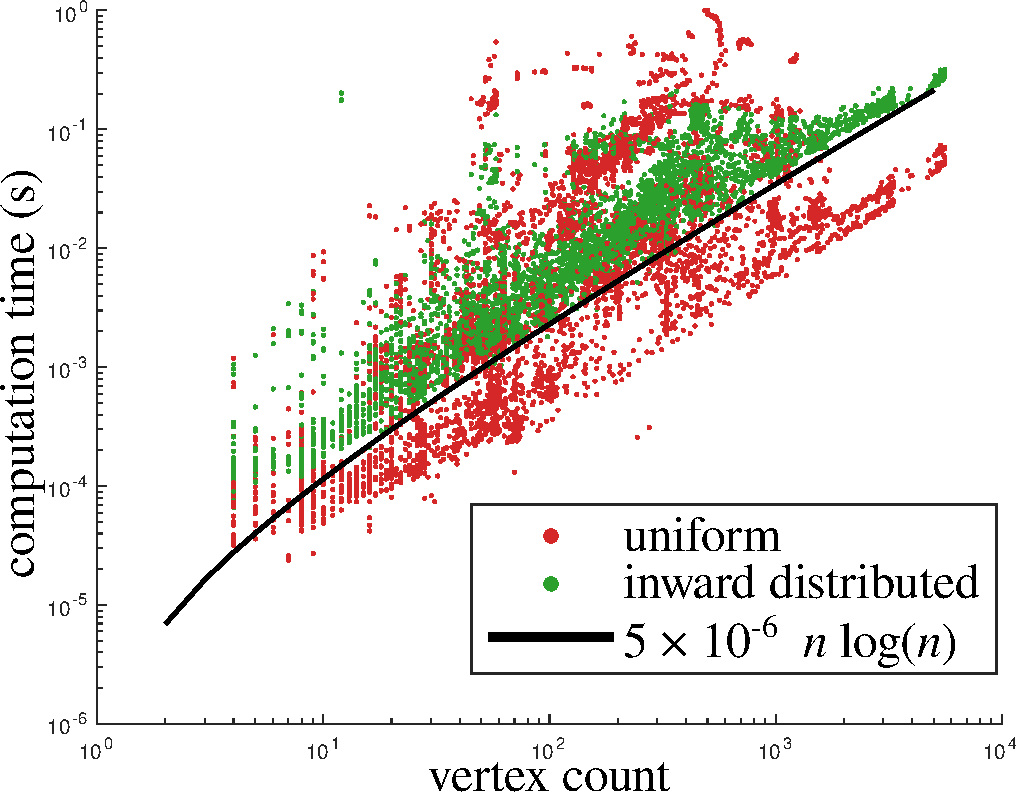
\includegraphics[width=\figwidth]{sources-validation-computime2.pdf}
\caption{Computation time}
\label{computime}
\end{subfigure}
\begin{subfigure}{\figwidth}\centering
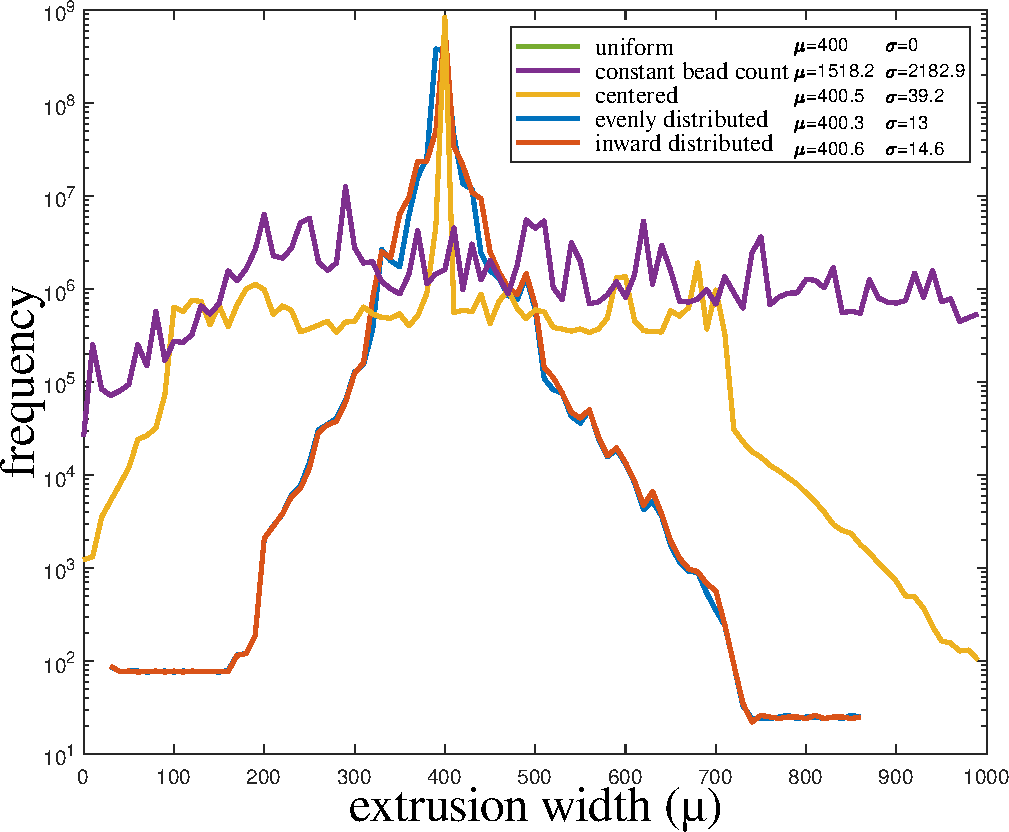
\includegraphics[height=\figheight]{sources-validation-widthHistogram.pdf}
%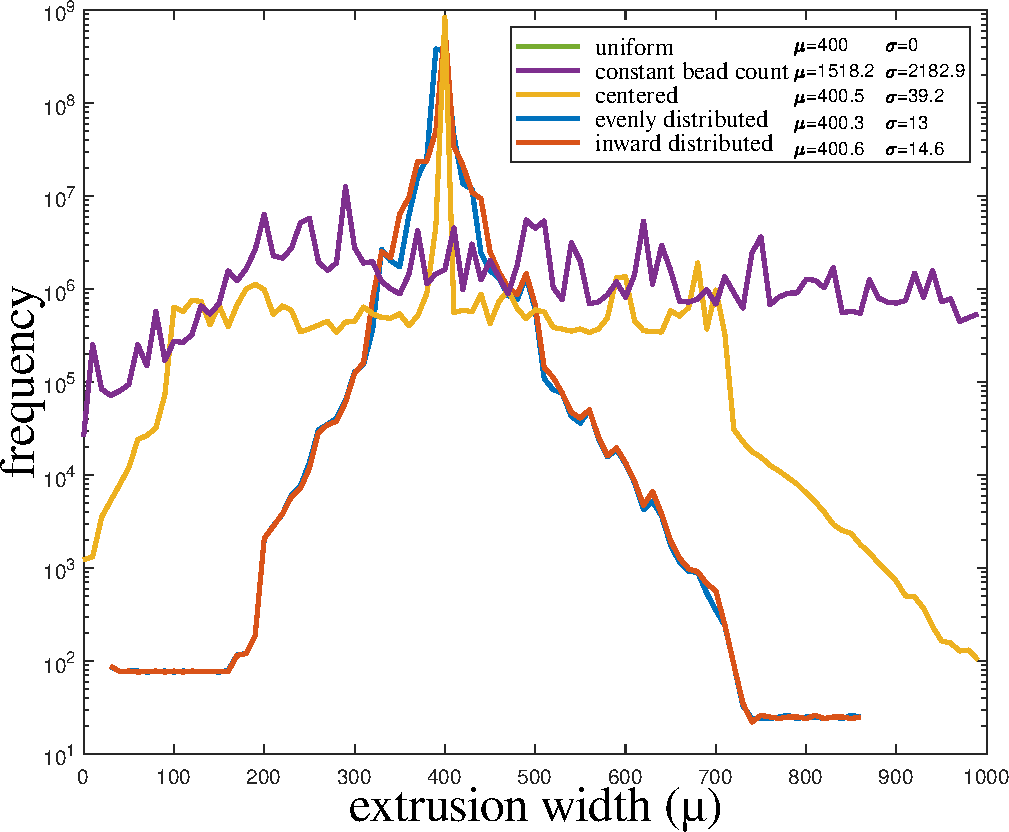
\includegraphics[width=\figwidth]{sources-validation-widthHistogram.pdf}
\caption{Extrusion widths}
\label{widthHistogram}
\end{subfigure}
\begin{subfigure}{\figwidth}\centering
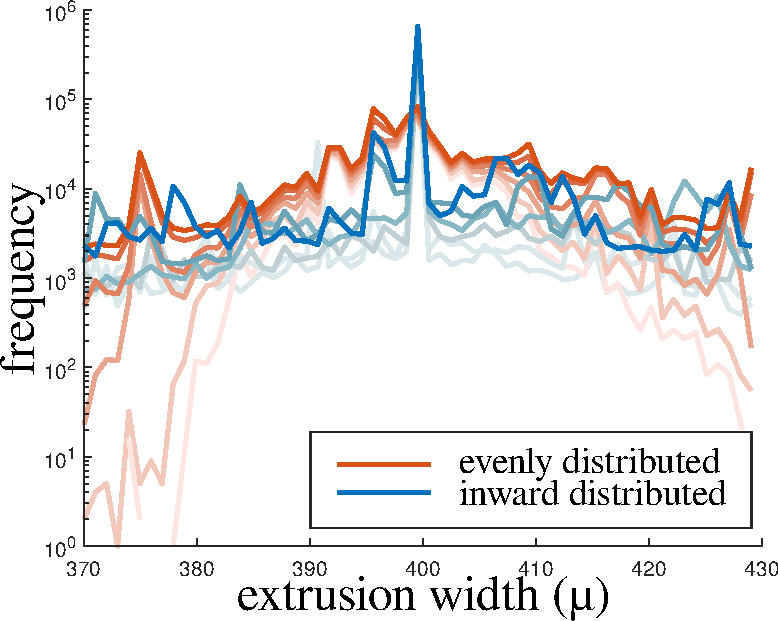
\includegraphics[height=\figheight]{sources-validation-indexedwidths2.pdf}
%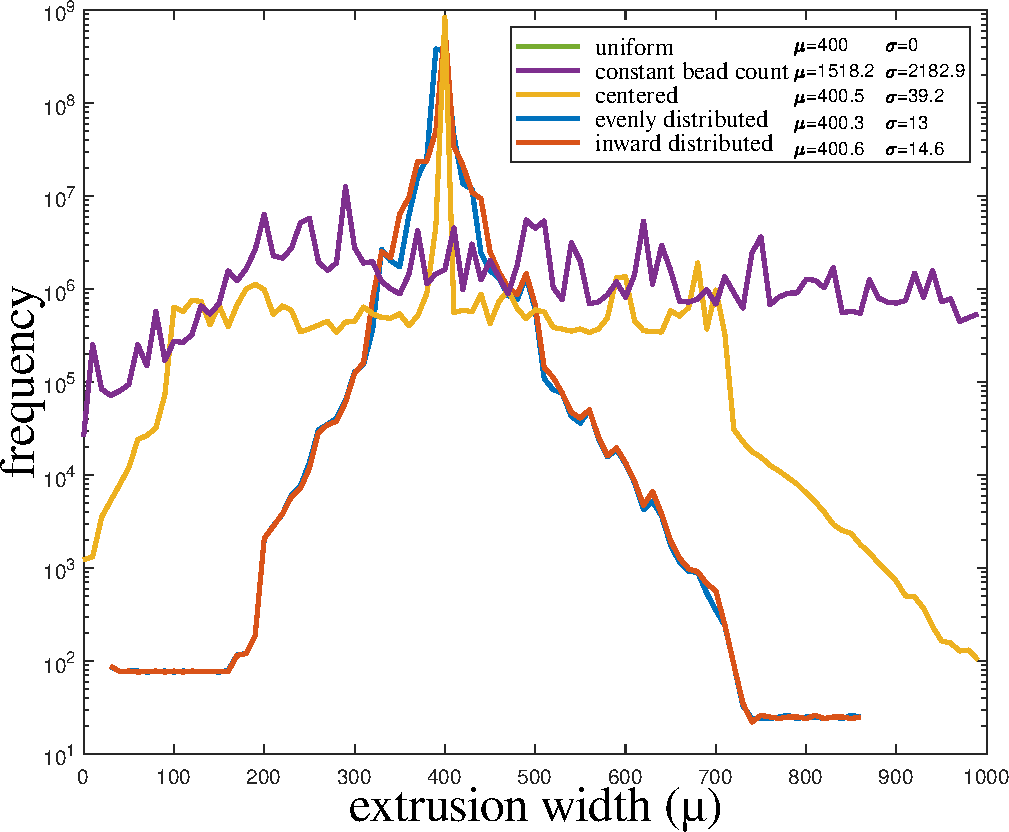
\includegraphics[width=\figwidth]{sources-validation-widthHistogram.pdf}
\caption{Extrusion width per index}
\label{widthIndexedHistogram}
\end{subfigure}
\begin{subfigure}{\figwidth}\centering
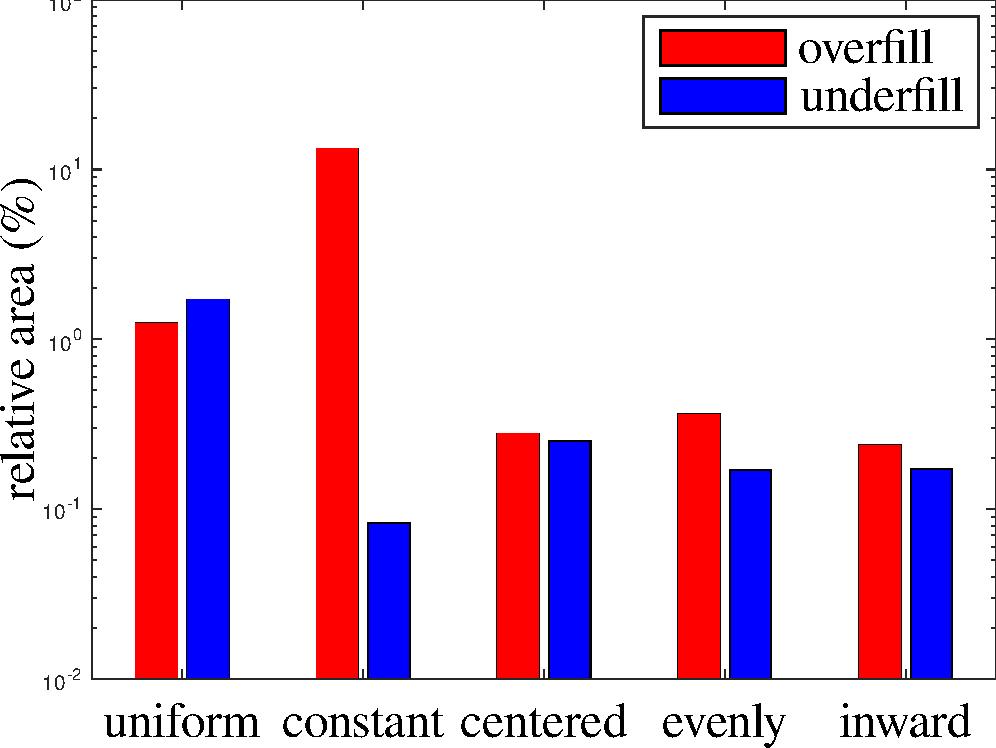
\includegraphics[height=\figheight]{sources-validation-overunderfill.pdf}
%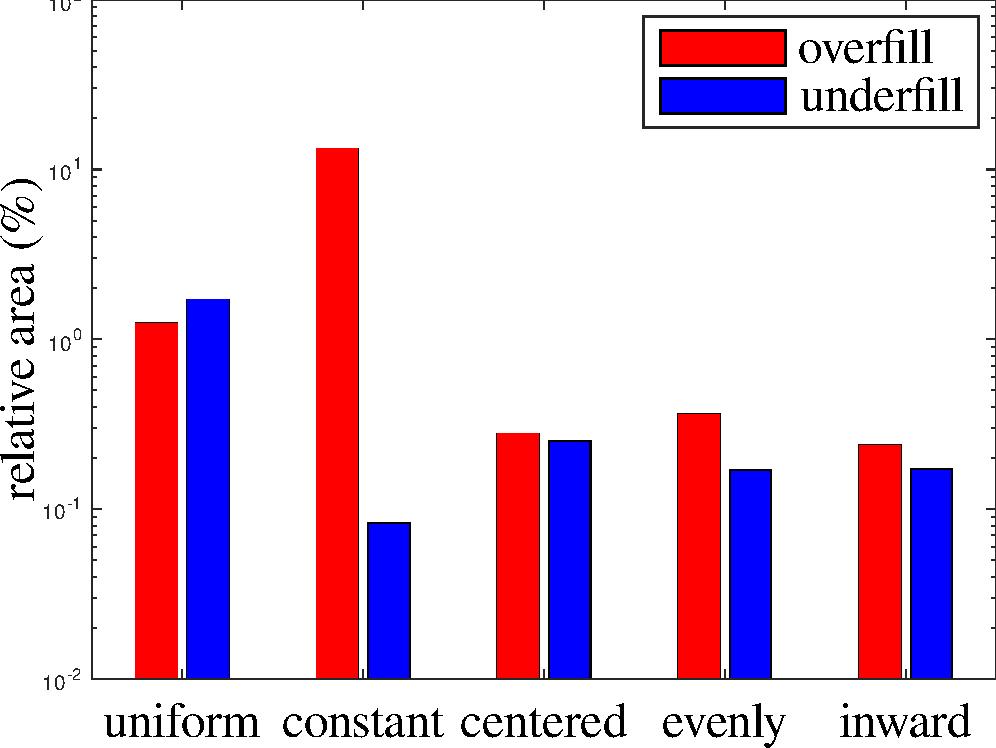
\includegraphics[width=\figwidth]{sources-validation-overunderfill.pdf}
\caption{Over- and underfill}
\label{over_underfill}
\end{subfigure}
\begin{subfigure}{\figwidth}\centering
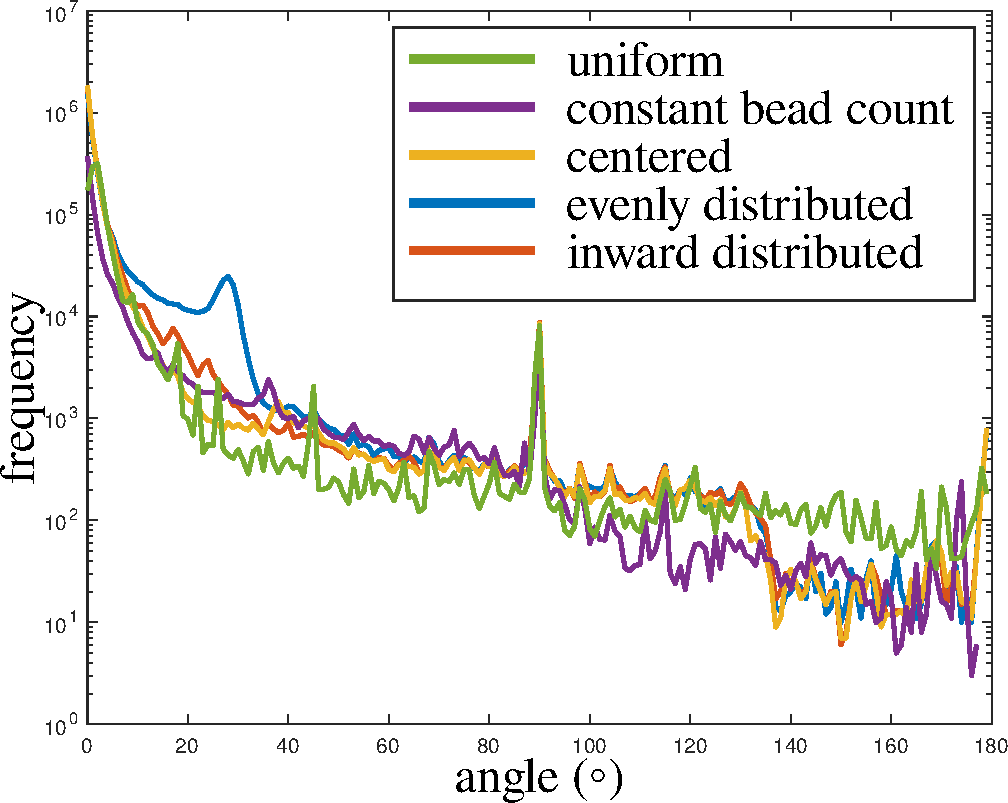
\includegraphics[height=\figheight]{sources-validation-smoothness.pdf}
%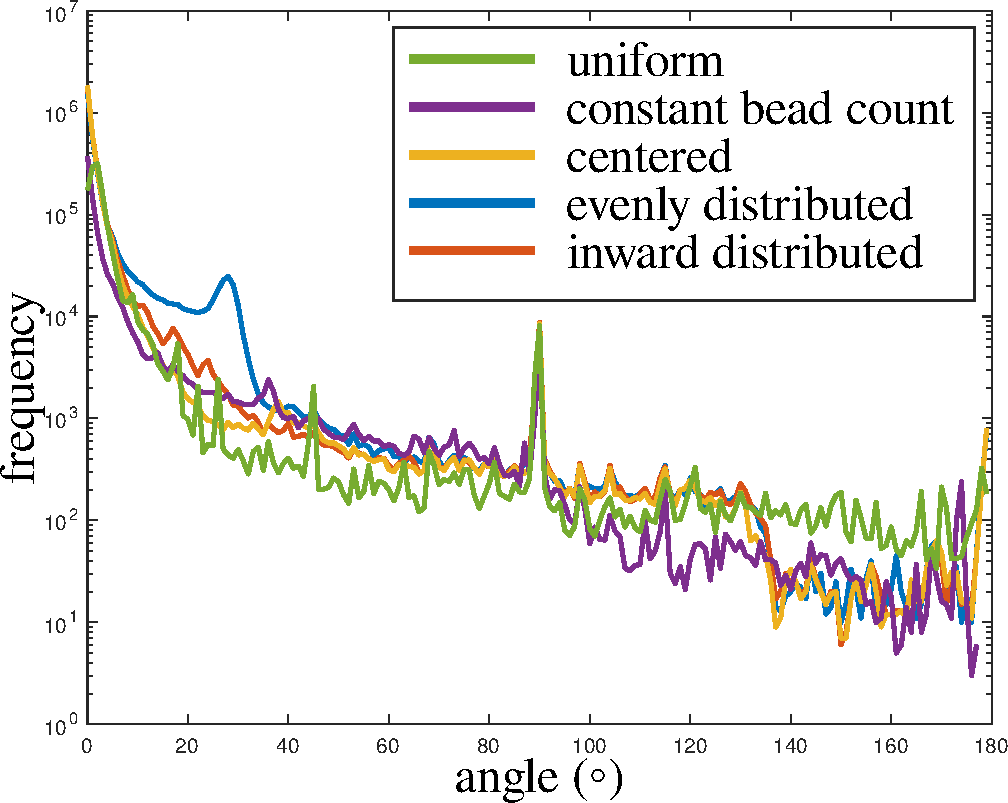
\includegraphics[width=\figwidth]{sources-validation-smoothness.pdf}
\caption{Site angles}
\label{smoothness}
\end{subfigure}
\begin{subfigure}{\figwidth}\centering
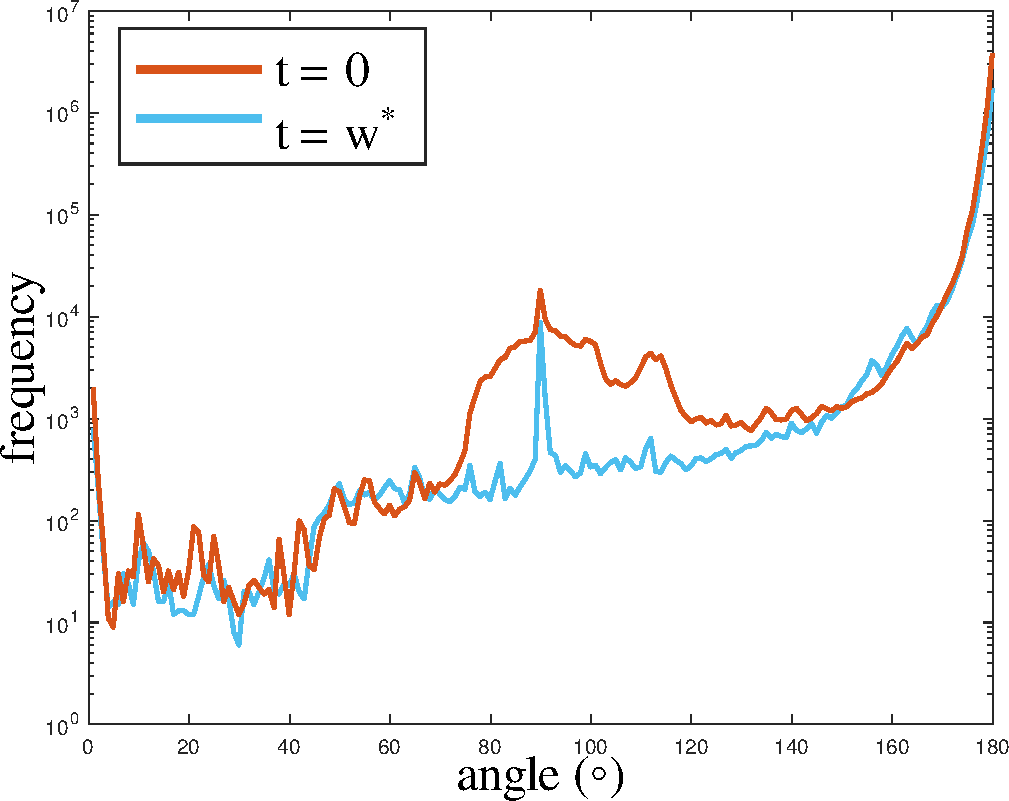
\includegraphics[height=\figheight]{sources-validation-smoothnessNoTransition.pdf}
%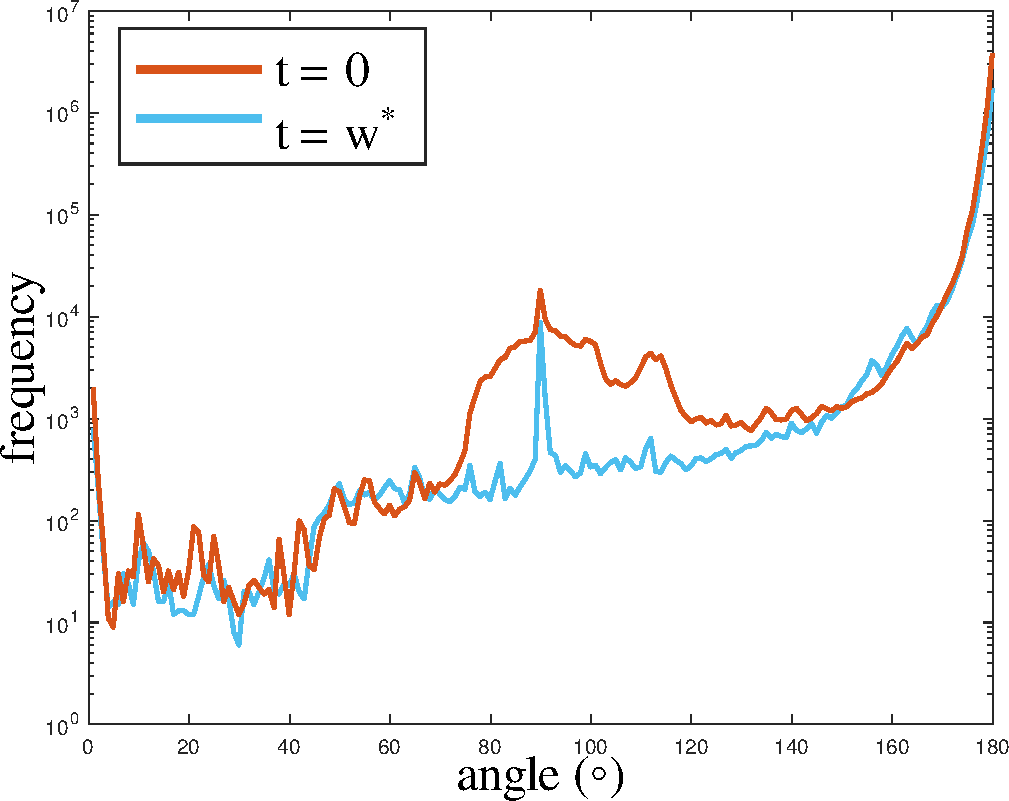
\includegraphics[width=\figwidth]{sources-validation-smoothnessNoTransition.pdf}
\caption{Site angles (inward distributed)}
\label{smoothnessNoTransition}
\end{subfigure}


\caption{
Statistical analysis of the toolpaths from applying the uniform width technique and various beading schemes using our framework to a data set of 300 slices.
Note the use of a logarithmic scale on the Y-axes and on some of the X-axes as well.
}
\end{figure*}









\subsubsection{Uniformity}
We visualize the bead widths resulting from the different schemes in the bottom of \cref{visualized_accuracy}.
We calculated the mean and standard deviation of the bead width, sampled at \SI{1}{\micro\meter} along the toolpaths.
\cref{widthHistogram} shows the distribution of extrusion width for each scheme binned at intervals of \SI{10}{\micro\meter}.
We found that the mean width of the inward and evenly distributed schemes is close to preferred bead width of \SI{400}{\micro\meter}, while their standard deviation is lower than for the centered and constant bead count scheme. 
These results show that, while causing less overfill and underfill, inwards distributed and evenly distributed schemes deviate less or less often from the preferred bead width compared to the other schemes.
We compared the width uniformity of the 6 outer beads for the inward and evenly distributed schemes, the distribution of these extrusion widths is shown in \cref{widthIndexedHistogram}. 
The outer beads of the inward distributed scheme deviate less from the preferred width compared to the evenly distributed scheme.

\subsubsection{Smoothness of toolpaths}
In order to maintain a high printing speed, it is desirable that toolpaths have fewer and less sharp corners. 
We therefore measured the angle between consecutive extrusion segments generated by each scheme
and report on the occurrence of each angle in \cref{smoothness}.
All schemes show a higher number of corners for smaller angles with a peak towards \SI{180}{\degree} (straight).
We observe that compared to the uniform method our framework produces less acute angles which, but more obtuse angles.
The inward distributed scheme produces an order of magnitude less corners around \SI{150}{\degree}, compared to evenly distributed. 
We also investigated the effect of the transition regions on the smoothness of the toolpaths. 
\cref{smoothnessNoTransition} shows that introducing the transitions greatly reduces the number of corners around \SI{90}{\degree}. 

\subsubsection{Computational performance}
\cref{computime} plots the computation time against the vertex count of the layer for the full data set, comparing the uniform technique implemented using Clipper~\cite{johnson2014clipper} to our framework with the inward distributed scheme.
For polygonal shapes with as many as $10^4$ vertices, the computation for both approaches is less than 1 second, with our method being approximately five times that of the uniform technique.
These results could be improved upon by utilizing the locality inherent in our algorithms for parallelization on the GPU.

The computational complexity is limited by the generation of the Voronoi Diagram, which is $O(n \log n)$, where $n$ is the number of vertices in the input shape.
The other steps in our framework have a complexity of $O(m)$, where $m$ is the number of elements in the ST.
Therefore, the total running time of our algorithm is $O(n \log n)$.
Results in \cref{computime} confirm that both our framework and the uniform technique have an expected running time of approximately $5 \times 10^{-6} n \log n$ seconds.





\revise{
Test prints were performed on a custom FDM hardware setup, with a standard \SI{0.4}{\milli\meter} nozzle and a filament extrusion drive directly mounted on the print head.
The firmware of the printer employs \emph{linear advance} for accurately realizing adaptive deposition width:
gaining the extra pressure required to change to a wider bead is realized by 'advancing' an extra amount of filament into the physical system~\cite{tronvoll2019investigating}.
We set the preferred width to $w^* = \SI{0.6}{\milli\meter}$, to avoid fluttered printing of lines narrower than the nozzle size.
We used a layer thickness of \SI{0.2}{\milli\meter} and a movement speed of \SI{10}{\milli\meter\per\second}.

The prints are shown in \cref{prints}.
Because of inaccuracies in the deposition control system some of the prints show defects.
Such defects are less prevalent for the inward distributed beading scheme than the other schemes.
The prints which employ the uniform offsets technique show a lot of underfill, which impacts the visual quality of the print.
Moreover, in the case of the regular honeycomb there are several fully disconnected hexagons, which means the object falls apart.
The difference between the centered and the inward distributed schemes is less pronounced.
We can still see some loosely connected extrusion segments in both, which is attributable to inaccuracies in the extrusion system.
However, the middle of \cref{wedge_print} exhibits more defects in the regions where the centered scheme produces extreme bead widths.
The bottom print shows that the inward distributed beading scheme produces smoother prints with less defects.


\begin{figure}
\centering
\begin{subfigure}{\columnwidth}\centering
\setlength{\figwidth}{\columnwidth}
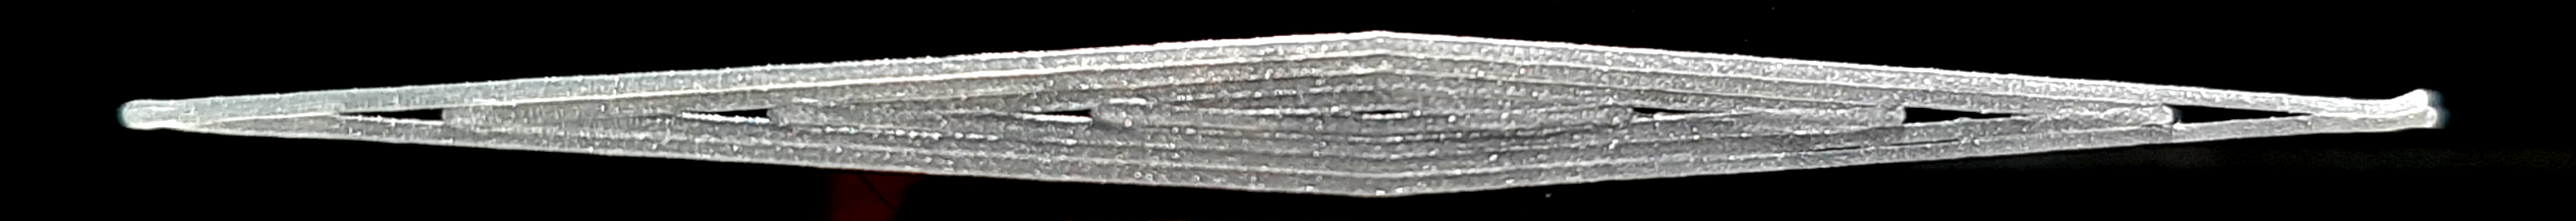
\includegraphics[width=\figwidth]{sources-applications-P3-print-wedge-naive-edited.png}
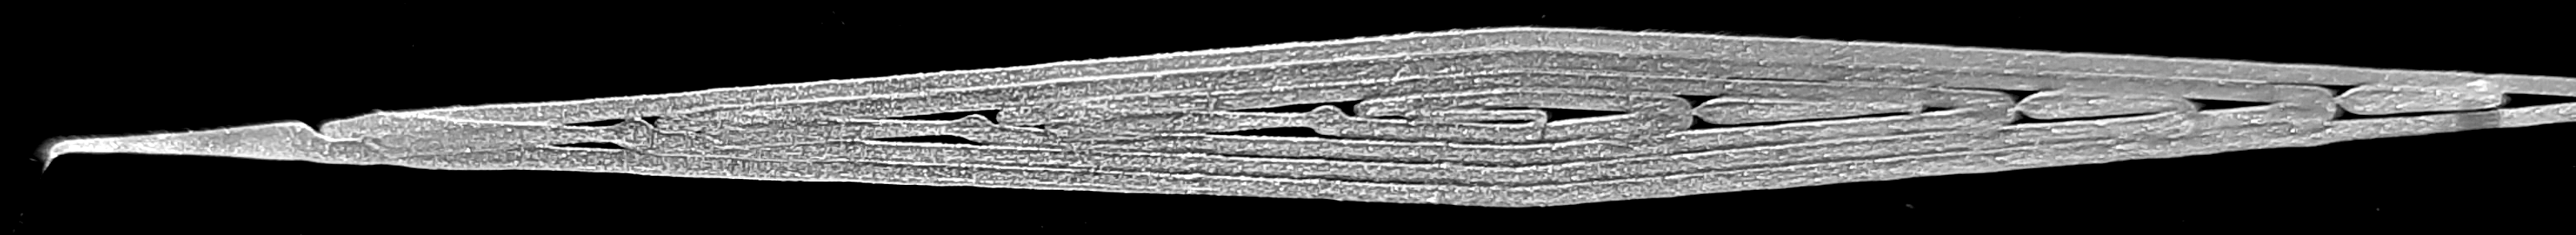
\includegraphics[width=\figwidth]{sources-applications-P3-print-wedge-center-edited.png}
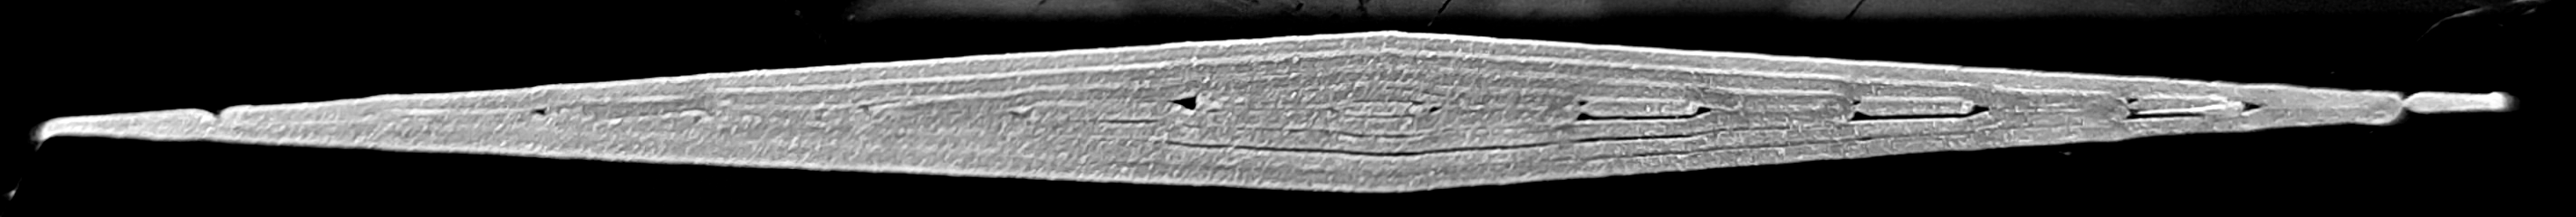
\includegraphics[width=\figwidth]{sources-applications-P3-print-wedge-inward-edited.png}
\caption{Uniform (top), centered (mid) and inward distributed (bottom)}\label{wedge_print}
\end{subfigure}
\setlength{\figheight}{.38\columnwidth}
\setlength{\figheightTwo}{.47\columnwidth}
\setlength{\figwidth}{0.32\columnwidth}
\begin{subfigure}{\figwidth}\centering
%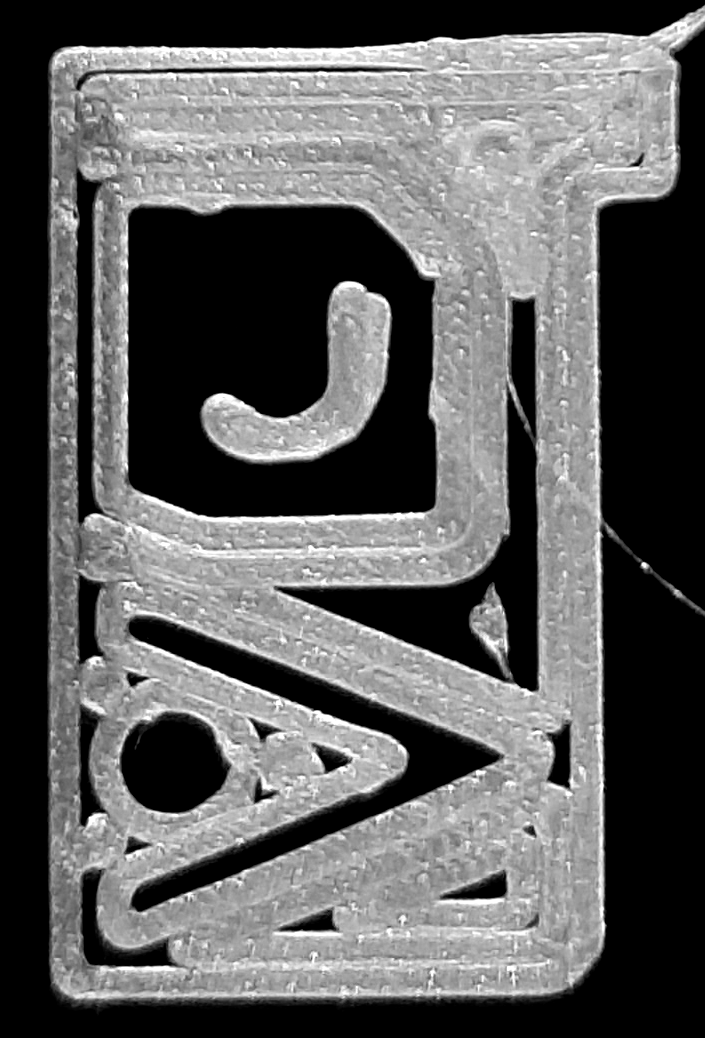
\includegraphics[height=\figheightTwo]{sources-applications-gMAT-naive.png}
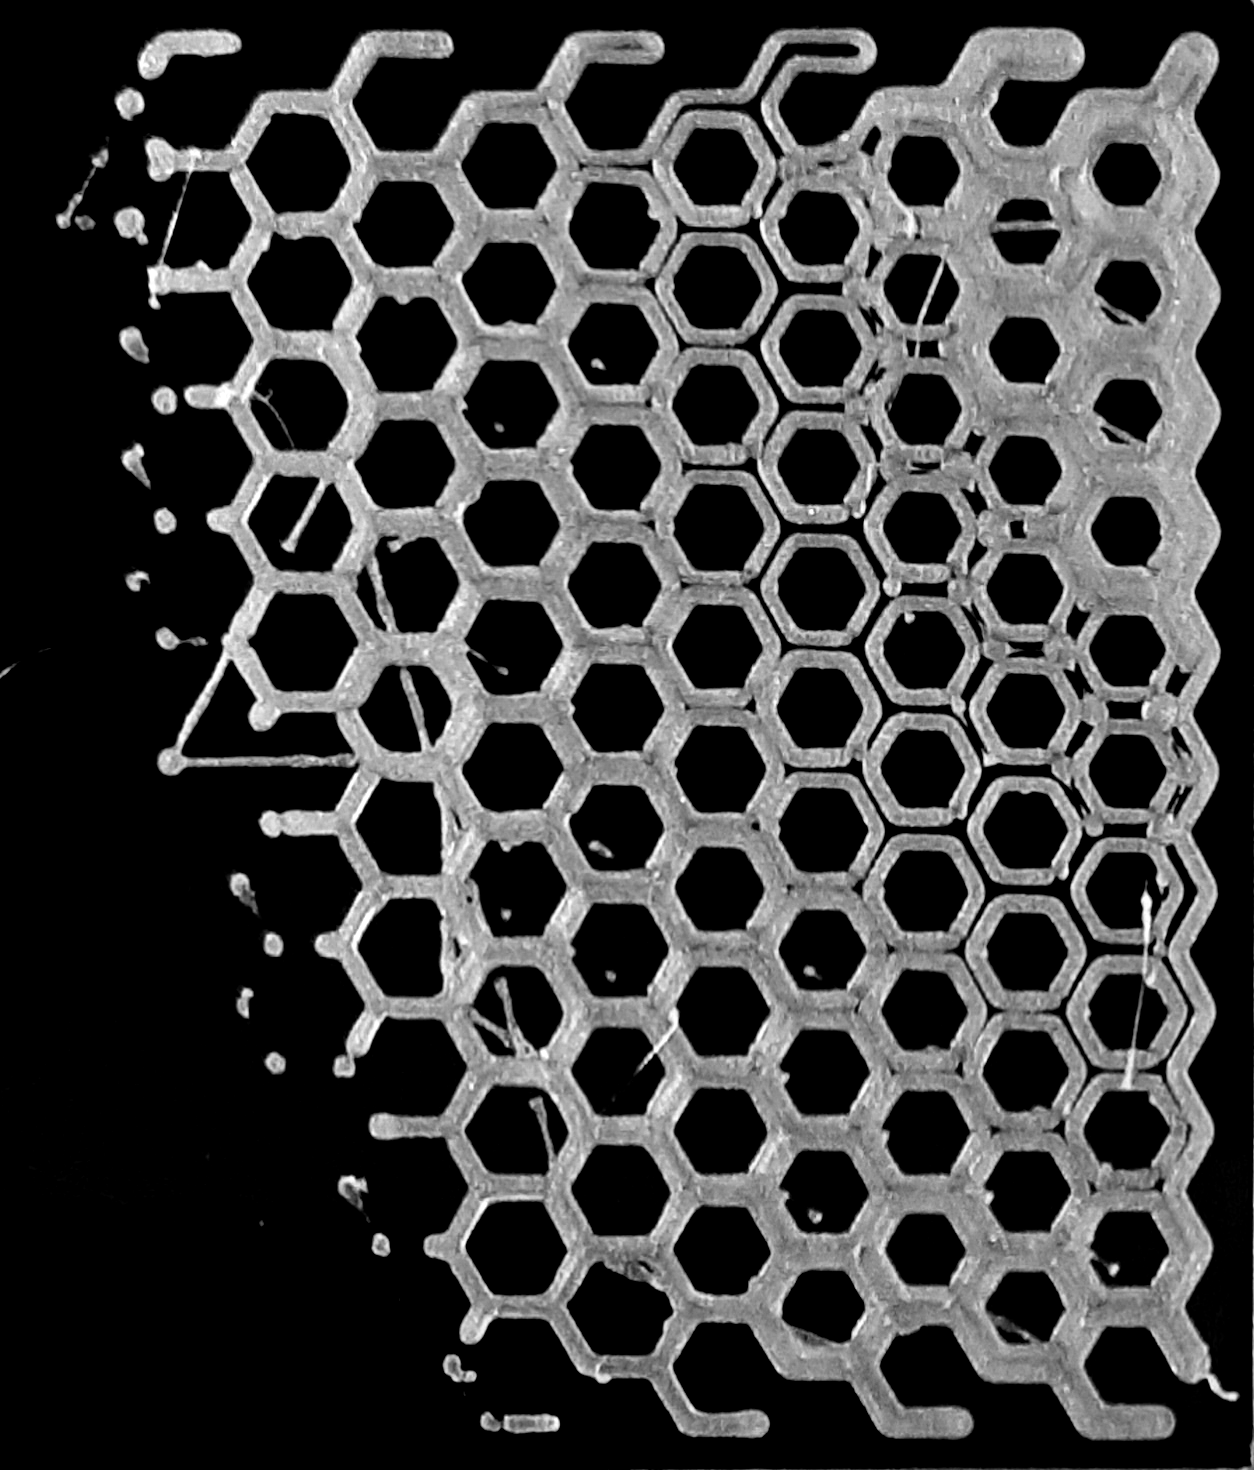
\includegraphics[height=\figheight]{sources-applications-P3-print-hex-naive-edited.png}

\includegraphics[width=\figwidth]{sources-applications-P3-print-UM-naive-edited.png}
\caption{Uniform}\label{print_naive}
\end{subfigure}
\begin{subfigure}{\figwidth}\centering
%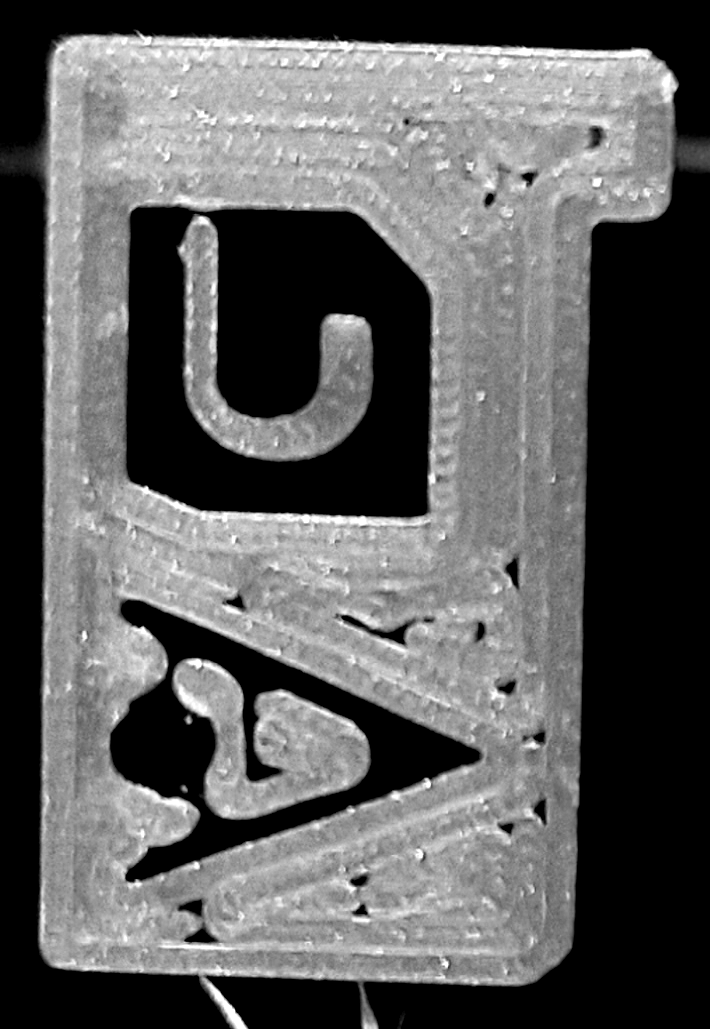
\includegraphics[height=\figheightTwo]{sources-applications-gMAT-center.png}
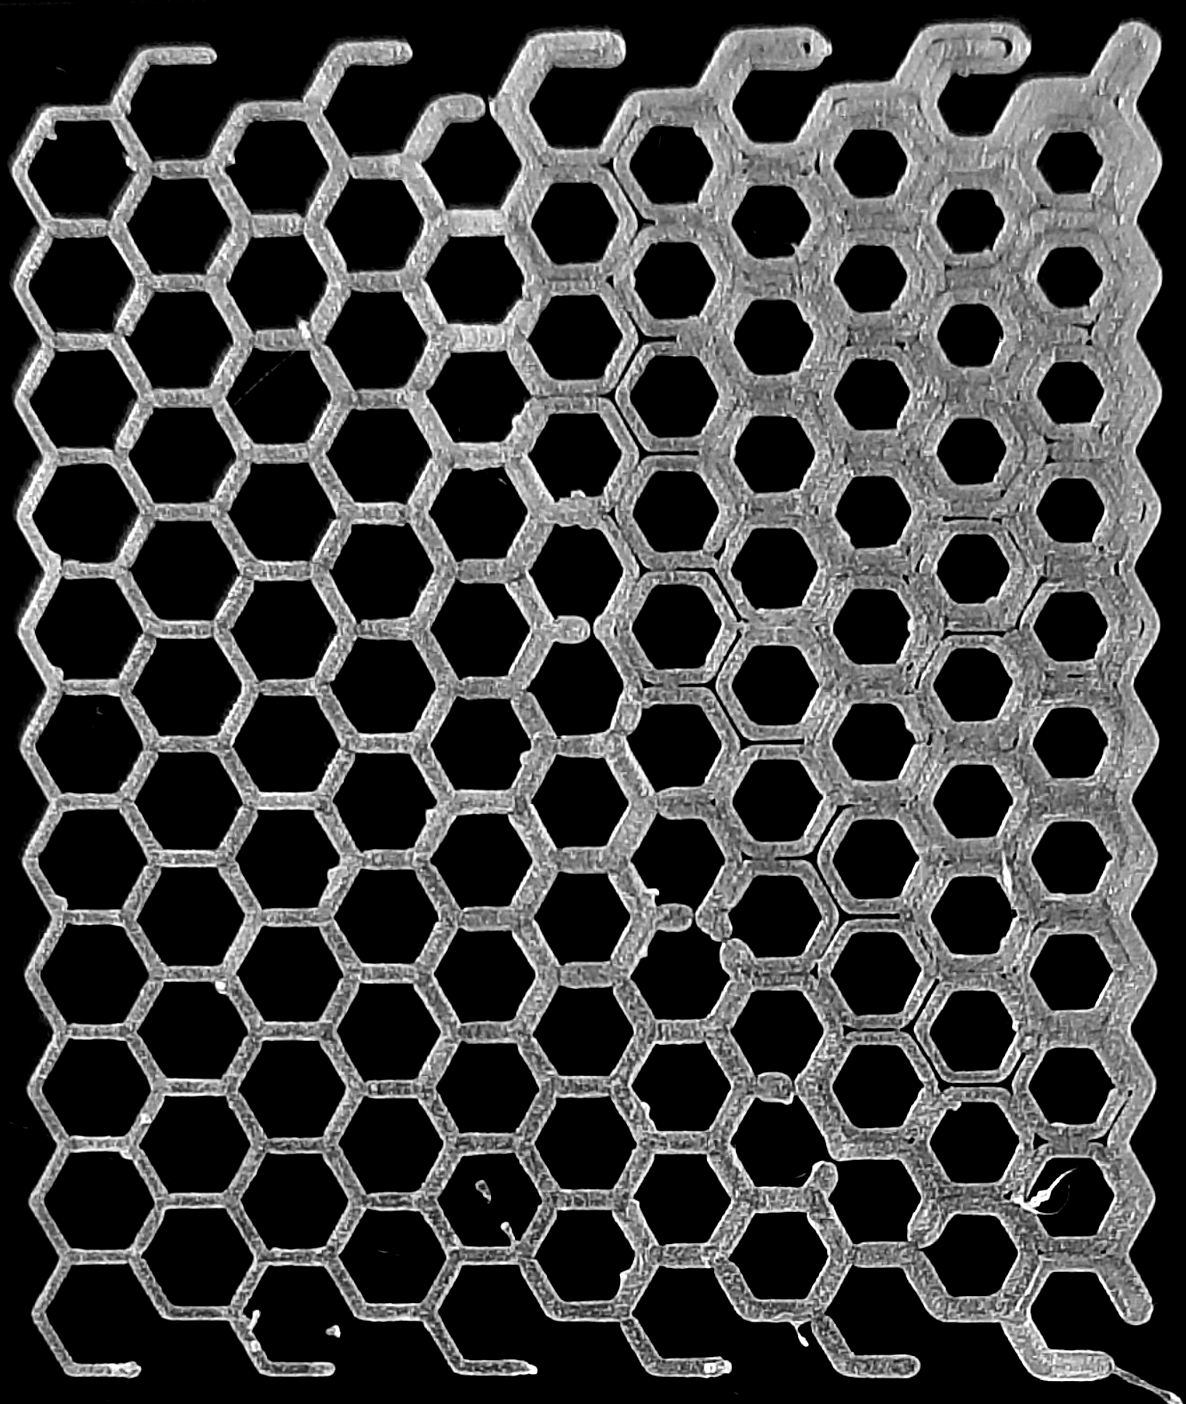
\includegraphics[height=\figheight]{sources-applications-P3-print-hex-center-edited.png}

\includegraphics[width=\figwidth]{sources-applications-P3-print-UM-center-edited.png}
\caption{Centered}\label{print_center}
\end{subfigure}
\begin{subfigure}{\figwidth}\centering
%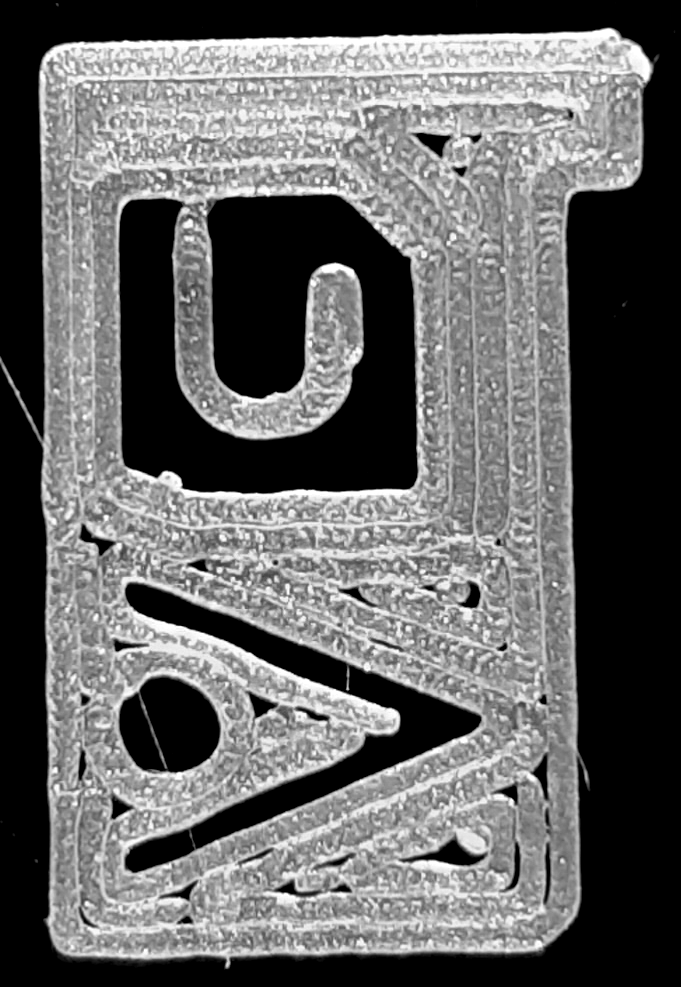
\includegraphics[height=\figheightTwo]{sources-applications-gMAT-inward.png}
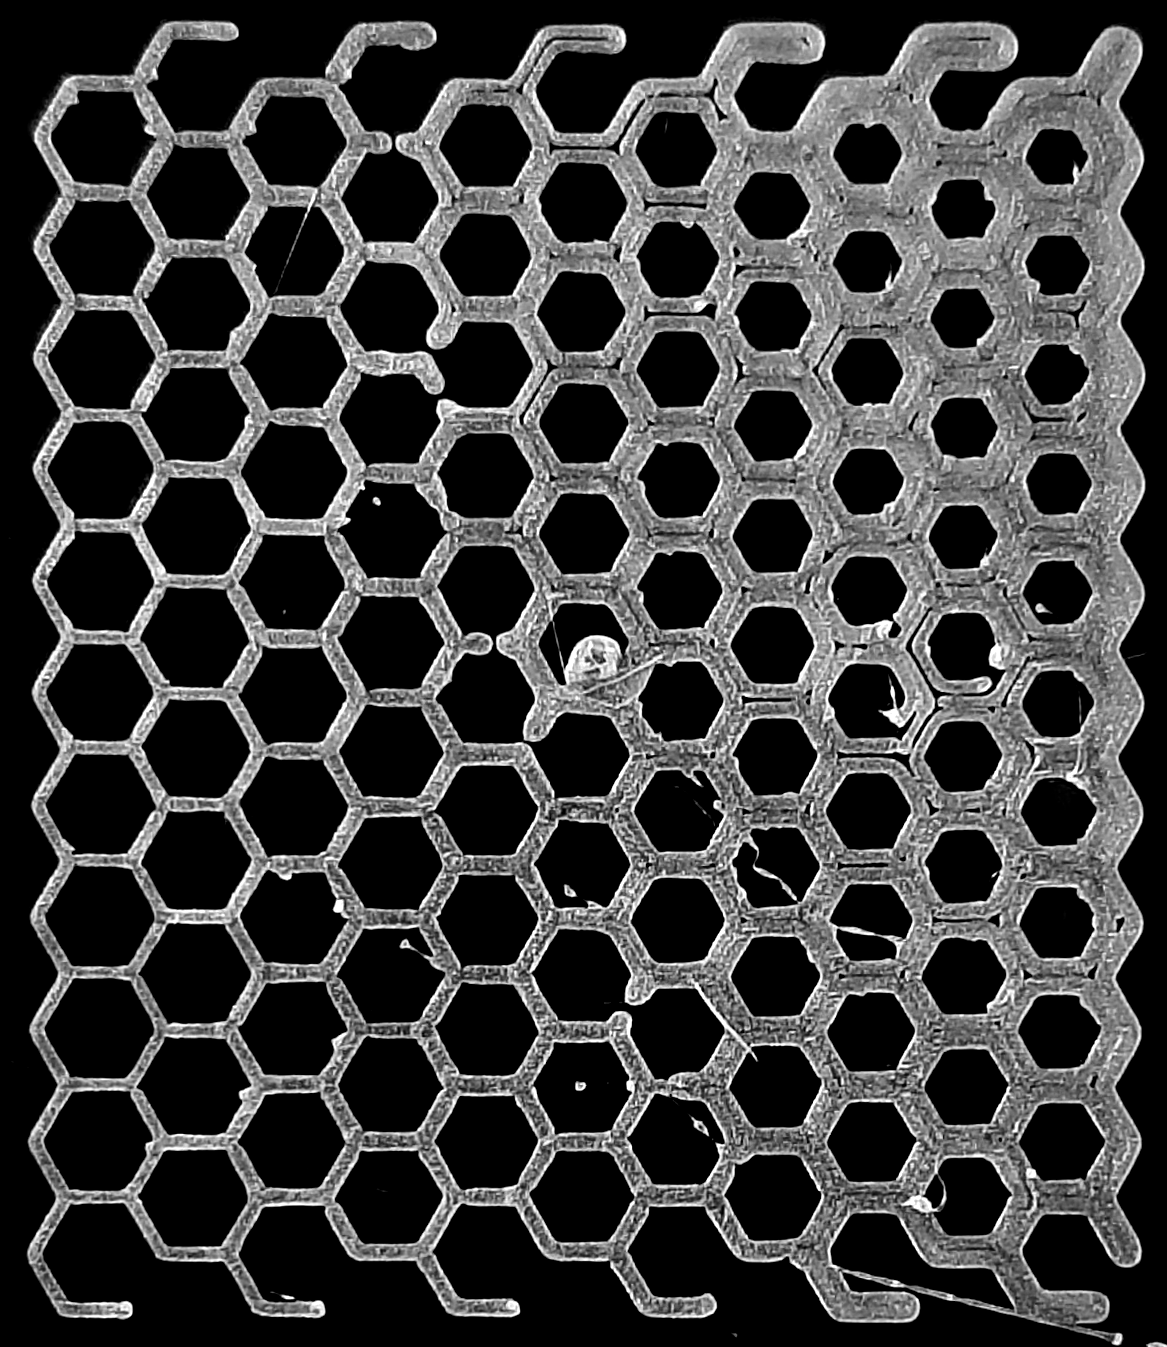
\includegraphics[height=\figheight]{sources-applications-P3-print-hex-inward-edited.png}

\includegraphics[width=\figwidth]{sources-applications-P3-print-UM-inward-edited.png}
\caption{Inward distributed}\label{print_inward}
\end{subfigure}
\caption{
Test shapes printed using the uniform scheme, centered scheme and the inward distributed scheme.
The uniform technique produces distinct underfill areas.
The centered scheme shows some defects due to inaccurate control of extreme deposition widths.
The inward distributed scheme produces the least defects.
}
\label{prints}
\end{figure}
}{}









%We therefore visualize include a semi-circle with a diameter equal to the starting width in the one end, and exclude it at the other end, because it will be included in the next extrusion segment.


